\documentclass{standalone}
\usepackage{tikz}
\usetikzlibrary{patterns, angles}
\usepackage{circuitikz}

\begin{document}
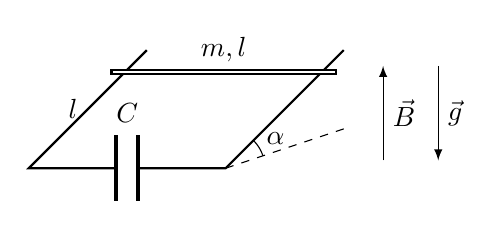
\begin{tikzpicture}
	\draw [arrows={-latex}] (4.5,0.1) -- (4.5, 1.3) node [midway, right] {$\vec{B}$};
	\draw [arrows={-latex}] (5.2,1.3) -- (5.2, 0.1) node [midway, right] {$\vec{g}$};
	\draw [thick] (1.5,1.5) -- (0,0) node [midway, left] {$l$} to [capacitor={$C$}] (2.5,0) to (4,1.5);
	\draw [thick, fill=white] (1.05, 1.2) rectangle (3.9,1.25) node [above=0pt, midway] {$m, l$};
	\draw [dashed] (2.5,0) -- (4,0.5);
	\coordinate (O) at (4,1.5);
	\coordinate (B) at (2.5,0);
	\coordinate (C) at (4,0.5);
	\pic [draw, -, angle eccentricity=1.5] {angle = C--B--O};
	\node [right=18pt, above=5pt] at (B) {$\alpha$};
	
\end{tikzpicture}
\end{document}